% Design
\section{Design}

\subsection{Package-Struktur}

Die Package-Struktur wird vom Sencha Touch 2 Framework vorgegeben. Sie entspricht grundsätzlich dem \gls{MVC}-Layout.
Speziell daran ist das Konzept der \emph{Stores}, welche einen beliebigen Datenspeicher abstrahieren.
Stores sind an ein \emph{Model} gebunden, welches die Struktur der gespeicherten Daten vorgibt.

Zusätzlich sind sie über einen \emph{Proxy} mit der Datenquelle verbunden.
Dabei kann es sich beispielsweise um einen \gls{REST}-Webservice handeln oder den \gls{Local Storage} des Browsers.

In Abbildung \ref{image-kort-packagediagram} wird die Package-Struktur von \textsc{Kort} mit deren Abhängigkeiten gezeigt.

\begin{figure}[H]
	\centering
	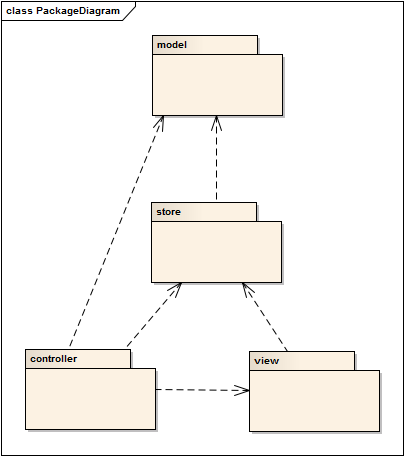
\includegraphics[scale=0.7]{images/uml/kort-packagediagram}
	\caption{Package-Struktur}
	\label{image-kort-packagediagram}
\end{figure}

\subsection{Controller-Package}

Die App wurde so gestaltet, dass jede Hauptansicht seinen eigenen Controller besitzt.
Dieser ist für die Steuerung der Benutzeroberfläche zuständig.

Die verschiedenen Controller lassen sich grob in drei Klassen einteilen.
Zum einen gibt es Controller für die einzelnen Tabs der Applikation (siehe Abbildung \ref{image-kort-classdiagram-controller} $\rightarrow$ \emph{main tab controllers}).
Zusätzlich haben einige Tabs eine Detailansicht, welche ebenfalls von einem eigenen Controller gesteuert wird (siehe Abbildung \ref{image-kort-classdiagram-controller} $\rightarrow$ \emph{detail controllers}).
Zuletzt gibt es eigenständige Controller für die Overlay-Komponenten, welche die gesamte Oberfläche der App verdecken (siehe Abbildung \ref{image-kort-classdiagram-controller} $\rightarrow$ \emph{overlay controllers}).

\begin{figure}[H]
	\centering
	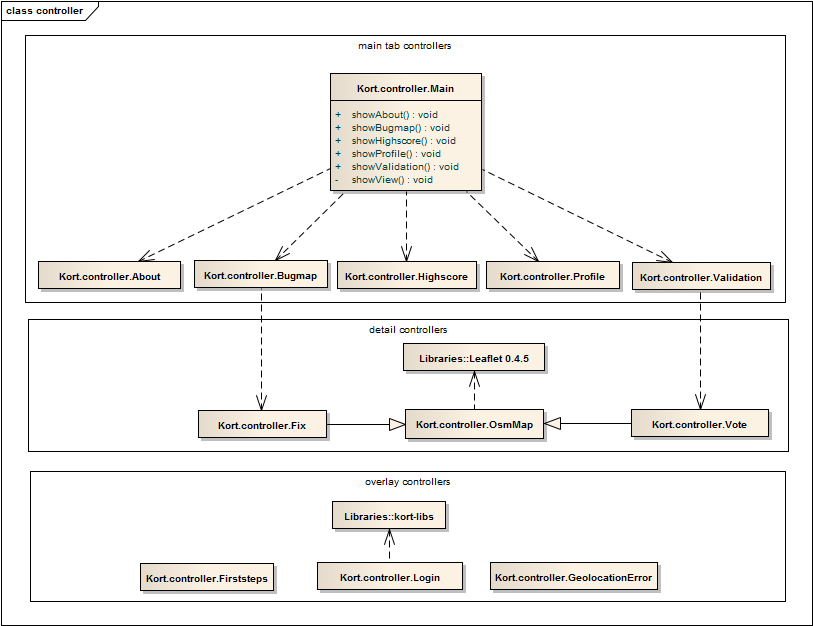
\includegraphics[width=\textwidth]{images/uml/kort-classdiagram-controller}
	\caption{Klassendiagramm der Controller}
	\label{image-kort-classdiagram-controller}
\end{figure}

\subsection{Store- und Model-Package}
\label{kort-store-model-package}

Die \emph{Stores} bilden die Datenspeicher in einer Sencha Touch Applikation.
Über ein \emph{Model} wird die jeweilige Struktur der gespeicherten Daten festgelegt.
Stores sind zudem über einen \emph{Proxy} mit der Datenquelle verbunden.
Im Falle von \textsc{Kort} wurden dafür ausschliesslich REST-Ressourcen verwendet.

\begin{figure}[H]
	\centering
	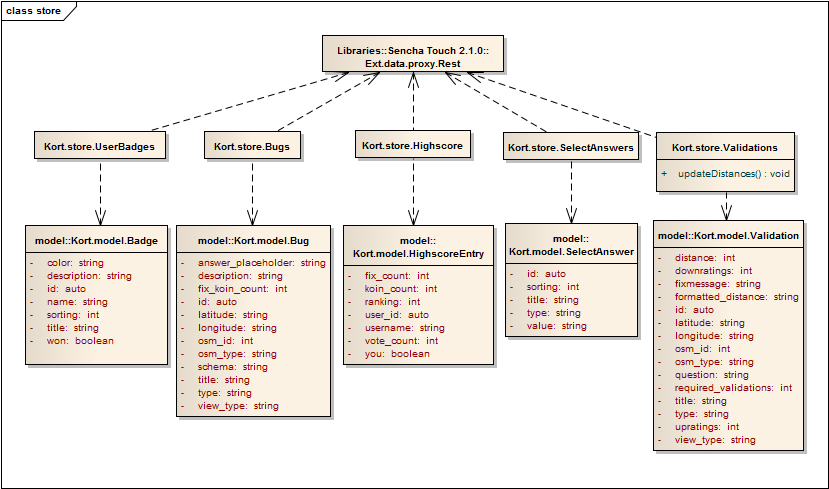
\includegraphics[width=\textwidth]{images/uml/kort-classdiagram-store}
	\caption{Klassendiagramm der Stores}
	\label{image-kort-classdiagram-store}
\end{figure}

\subsubsection{Models ohne Store}

Falls die Applikation jeweils nur eine Instanz eines \emph{Models} verwendet, können diese ohne einen Store direkt mit einem Proxy verbunden werden.
In \textsc{Kort} wurde dies für den eingeloggten Benutzer (User) sowie für die zu sendenden Datenpakete wie der Fehler-Lösung (Fix) und der Validierung (Vote) verwendet.

\begin{figure}[H]
	\centering
	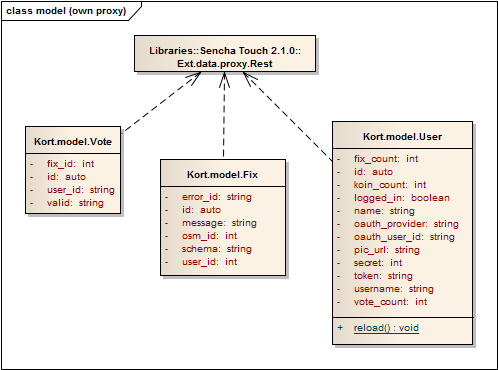
\includegraphics[scale=0.6]{images/uml/kort-classdiagram-model_own_proxy}
	\caption{Klassendiagramm der Models ohne Stores}
	\label{image-kort-classdiagram-model_own_proxy}
\end{figure}

\subsubsection{Speichern der Logininformationen}
Die Logininformationen des Benutzers werden im \gls{Local Storage} des Browsers abgelegt.
Der genau Ablauf wird in Abschnitt \ref{oauth} beschrieben.

\begin{figure}[H]
	\centering
	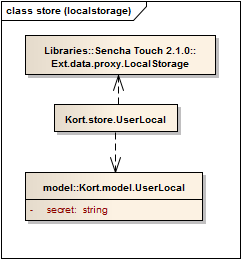
\includegraphics[scale=0.6]{images/uml/kort-classdiagram-store_localstorage}
	\caption{Speichern der Logininformationen über Local Storage}
	\label{image-kort-classdiagram-store_localstorage}
\end{figure}

\subsection{Aufbau der Benutzeroberfläche}
Jede Maske der Applikation befindet sich in einer eigenen View-Klasse.
Diese verschiedenen View-Klassen werden in der Hauptklasse \inlinecode{Kort.view.Main} inkludiert und angezeigt.

\begin{figure}[H]
	\centering
	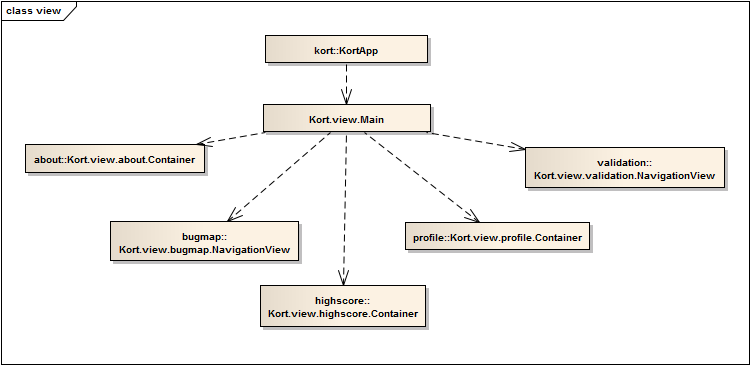
\includegraphics[width=\textwidth]{images/uml/kort-classdiagram-view}
	\caption{Aufbau der Benutzeroberfläche}
	\label{image-kort-classdiagram-view}
\end{figure}